\section{Modélisation}


	L'analyse de notre programme nous permet à présent d'avoir une vision plus précise des fonctionnalités de notre programme en vue de réaliser son diagramme de classe. Pour simplifier la modélisation et permettre une plus grande modularité de nos classe nous avons voulu utiliser aux maximums des patrons de conceptions. 

	\subsection{patron de Conception}
		\subsubsection{Fabrique : création de différents peuples}
		La création des peuples est assurée par le patron de conception créationnel \emph{Fabrique}. Ce patron de conception nous permettra de créer l'armée adéquate en fonction du peuple choisie par le joueur au lancement de la partie. 
		
		\subsubsection{Monteur : création d'une partie}
		La création d'une partie est assurée par le patron de conception \emph{Monteur}. Ce patron de conception nous permet de séparer la conception de l'objet Game de sa réprésentation. Ainsi, il sera plus facile de créer de nouveaux types de parties à l'avenir et l'on évite des recopies de codes entres les différentes type de parties réalisables.

%		\begin{figure}[h]
%		\begin{center}
%			\includegraphics[width=0.5\textwidth]{figure/UnitFactory.png}
%		\end{center}
%		\caption{Implémentations du plateau de jeu : patron de conception strategie}
%		\label{fig:strategy}
%	\end{figure}

		\subsubsection{Poids-Mouche : ne sert a rien}

		\subsubsection{Stratégie : création des différents type de carte}


%		\begin{figure}[h]
%			\begin{center}
%				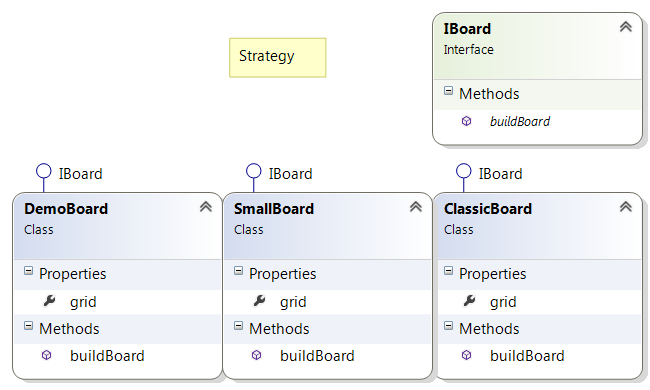
\includegraphics[width=0.5\textwidth]{figure/strategy.png}
%			\end{center}
%			\caption{Implémentations du plateau de jeu : patron de conception strategie}
%			\label{fig:strategy}
%		\end{figure}

		La création des cartes, de tailles fixes mais dont la composition des dalles est implémentée de maniére aléatoire, repose sur le patron de conception \emph{stratégie}. Ce patron de conception nous permet de choisir de manière précise l'algorithme de création de carte désiré. De plus, il permet une grande flexibilité pour définir de nouveaux types de cartes.



	\subsection{Diagramme de classe}


	\begin{figure}
		\begin{center}
			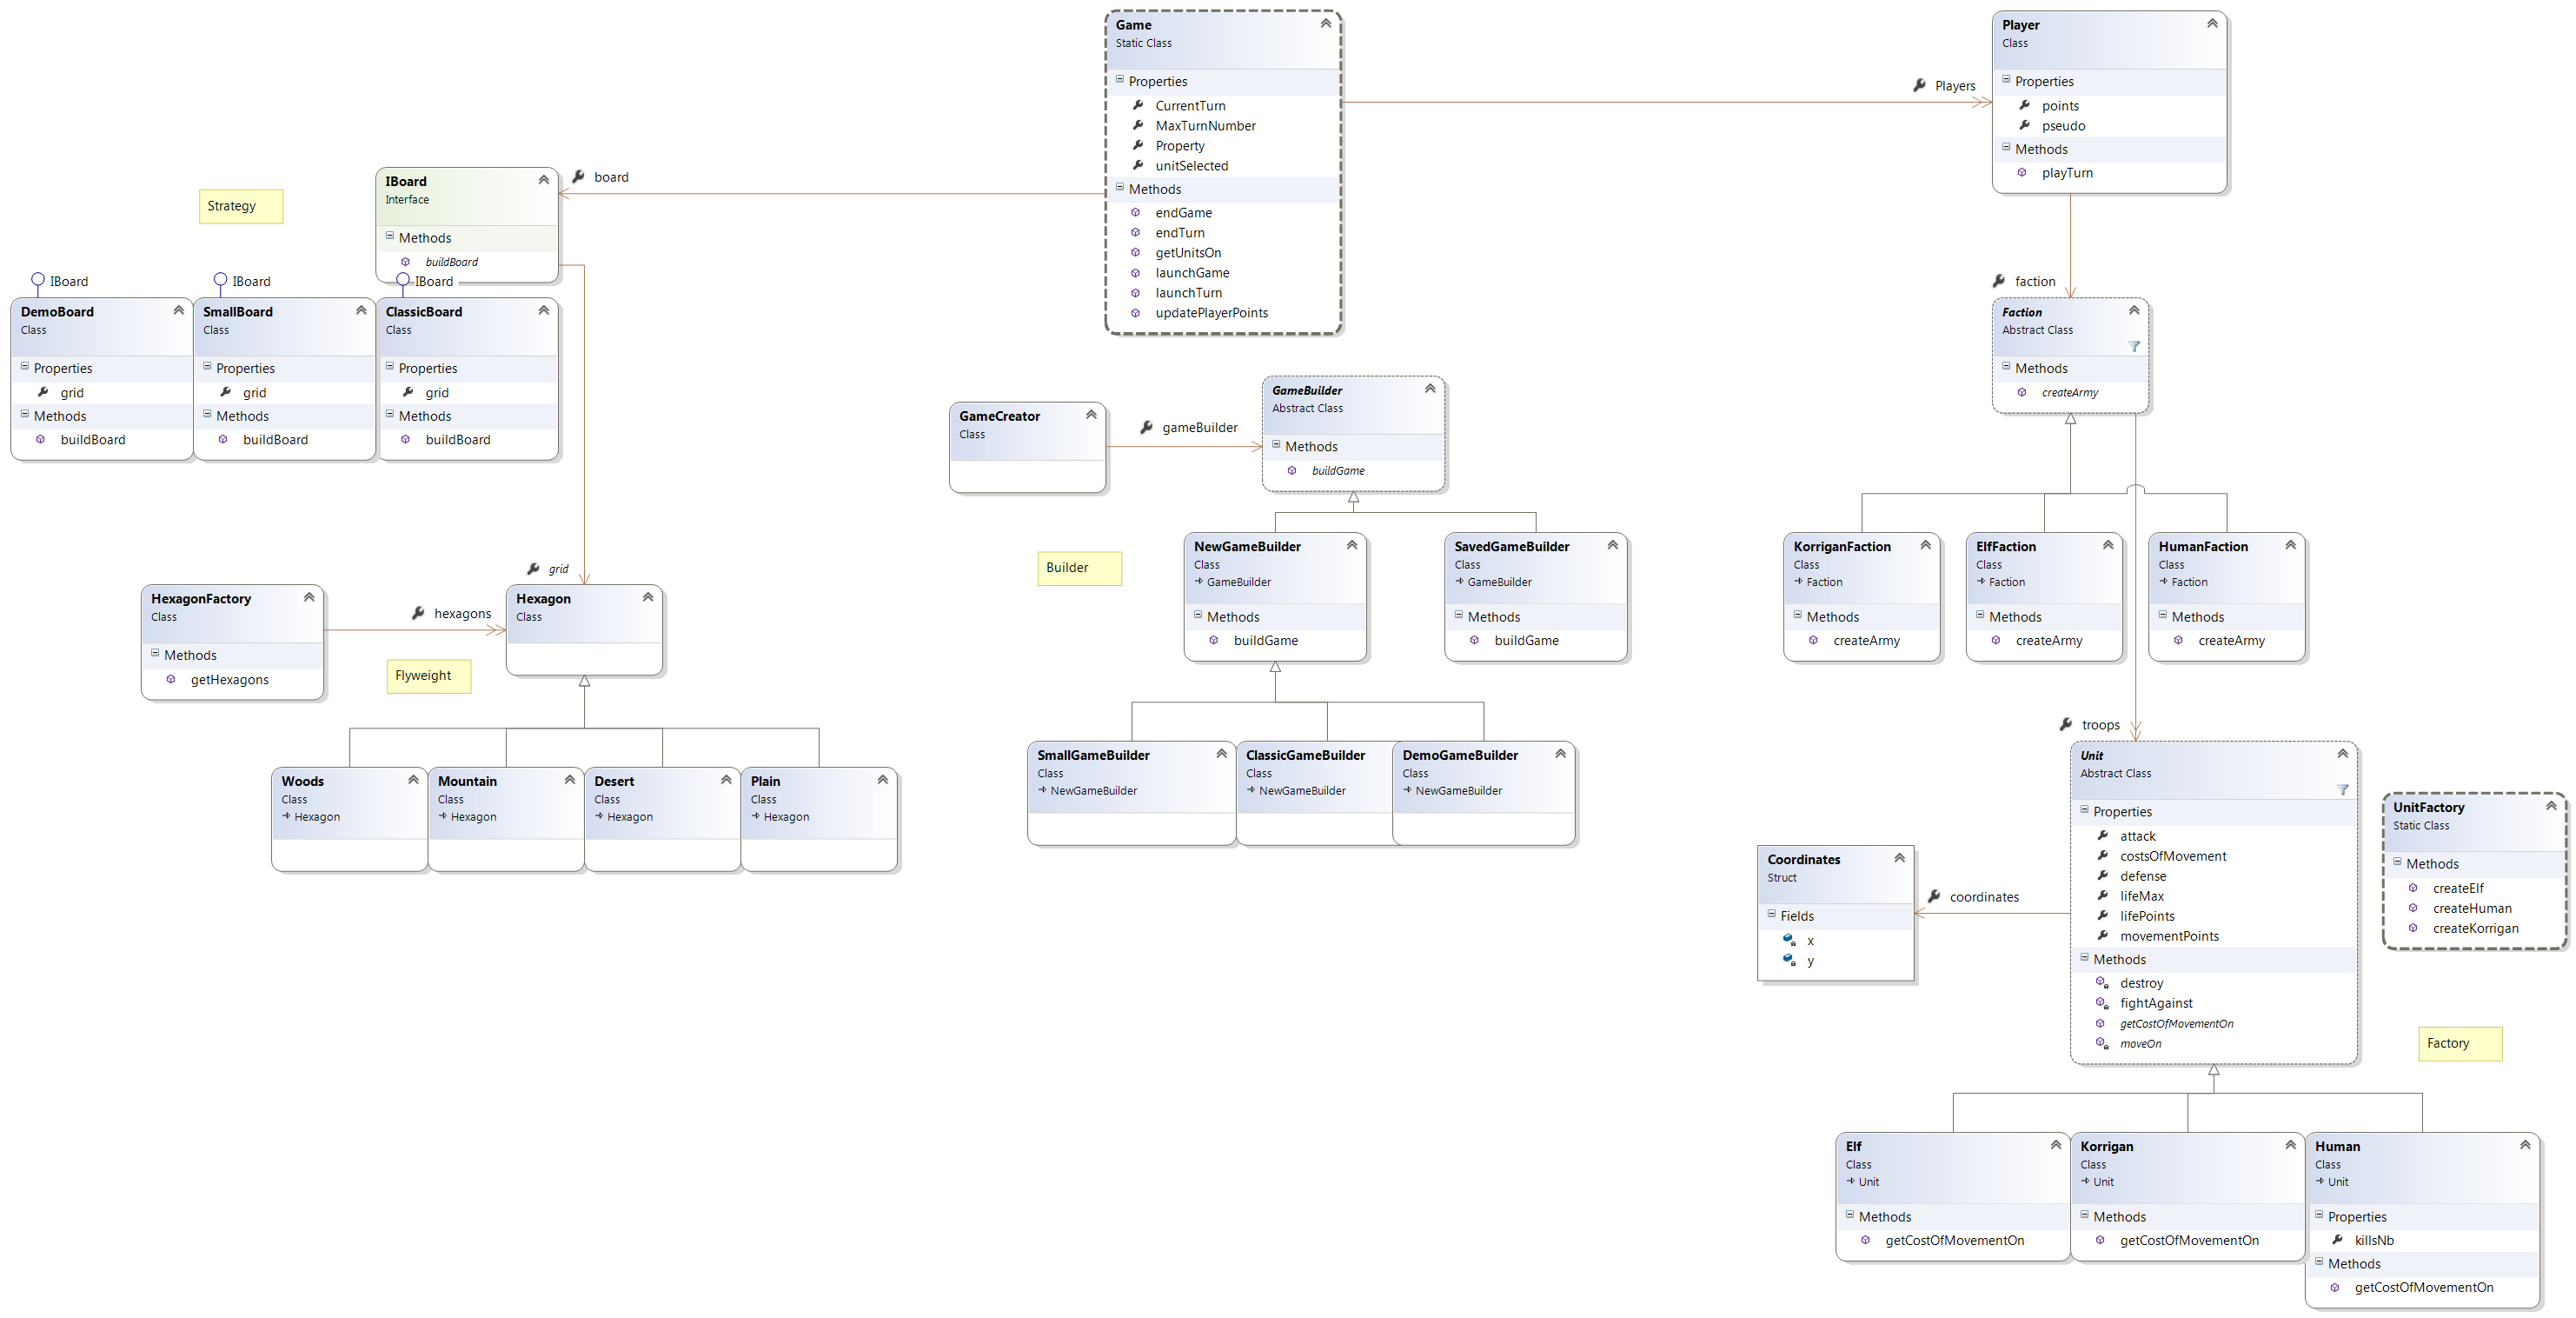
\includegraphics[width=0.5\textwidth]{figure/entire_class_diagram.png}
		\end{center}
		\caption{Diagrame de classe}
		\label{fig:planif}
	\end{figure}




